\documentclass[aspectratio=169]{beamer}
\usepackage[vietnamese]{babel} % Vietnamese in LaTeX
\usetheme{Madrid}
\usefonttheme{structurebold}
\usefonttheme[onlymath]{serif}

%\definecolor{BKTemplate}{rgb}{0.11765, 0.30588, 0.47451}
%\usecolortheme[named=BKTemplate]{structure}
\setbeamercolor{title}{fg=,bg=} 
\setbeamertemplate{caption}[numbered]

\usepackage{comment}
\usepackage[utf8]{inputenc}
\usepackage[T1]{fontenc}    % use 8-bit T1 fonts
\usepackage{url}            % simple URL typesetting
\usepackage{booktabs}       % professional-quality tables
\usepackage{amsfonts}       % blackboard math symbols
\usepackage{nicefrac}       % compact symbols for 1/2, etc.
\usepackage{microtype}      % microtypography
\usepackage{mathtools}
\usepackage{multicol}
\usepackage{comment}
\usepackage{forest}
\usepackage[linesnumbered, ruled]{algorithm2e}
\usepackage{algorithmic}
\usepackage{xcolor}
\usepackage{colortbl}
\usepackage{graphicx}
\usepackage{diagbox}
\usepackage{tikz}
\usepackage{subcaption}
% \captionsetup[subfigure]{labelsep=space}
\usepackage{amsmath}
\usepackage{dsfont}
\usepackage{stmaryrd}
\usepackage[style=authortitle,backend=bibtex]{biblatex}
\addbibresource{thesiscite.bib}

\renewcommand{\footnotesize}{\tiny}
\newcommand{\mathbi}[1]{\boldsymbol{#1}}
\newtheorem{proposition}{Proposition}

%------------------------------------------------------------
%This block of code defines the information to appear in the
%Title page
\title[Thiết kế hệ thống nhúng] %optional
{\vspace*{1cm}\\\textbf{BÁO CÁO BÀI TẬP LỚN}\\\textbf{THIẾT KẾ HỆ THỐNG NHÚNG}\\\textbf{MÁY CHƠI GAME CẦM TAY BKONSOLE}}

\subtitle{}

\author[Nhóm 9] % (optional)
{GVHD: ThS. Nguyễn Phan Hải Phú}


\institute[HCMUT] % (optional)
{
    ĐẠI HỌC QUỐC GIA THÀNH PHỐ HỒ CHÍ MINH\\
    TRƯỜNG ĐẠI HỌC BÁCH KHOA\\
    KHOA ĐIỆN - ĐIỆN TỬ \\
    BỘ MÔN ĐIỆN TỬ
}

\date[\today] % (optional)
{Thành phố Hồ Chí Minh - \today}

%End of title page configuration block
%------------------------------------------------------------



%------------------------------------------------------------
%The next block of commands puts the table of contents at the 
%beginning of each section and highlights the current section:

\AtBeginSection[]
{
  \begin{frame}
    \frametitle{Table of Contents}
    \tableofcontents[currentsection]
  \end{frame}
}
%------------------------------------------------------------


\begin{document}

% The next statement creates the title page.
\setbeamertemplate{background canvas}{
	
\includegraphics[width=\paperwidth,height=\paperheight]{images/FrontBackground.pdf}
}
\begin{frame}[plain]
\titlepage
\end{frame}


% Set background for all pages
\setbeamertemplate{background canvas}{
	
\includegraphics[width=\paperwidth,height=\paperheight]{images/Background.pdf}
}

\begin{frame}
\begin{table}[h!]
\centering
\begin{tabular}{|c|c|c|c|c|}
\hline
\textbf{Họ và Tên} & \textbf{MSSV} & \textbf{Nhiệm vụ phân công} & \textbf{Phần trăm công việc} \\ \hline
Vũ Nhật Huy & 2311267 & Thi công, thiết kế phần cứng & $100\%$ \\ \hline
Nguyễn Minh Thuận & 2313355 & Thi công phần cứng & $100\%$ \\ \hline
Thái Đức Thiên & 2313222 & Thiết kế, thực hiện phần mềm & $100\%$ \\ \hline
Đặng Minh Trí & 2313589 & Thực hiện phần mềm & $100\%$ \\ \hline
\end{tabular}
\end{table}
\end{frame}

%---------------------------------------------------------
%This block of code is for the table of contents after
%the title page
\begin{frame}
\frametitle{Mục lục}
\tableofcontents
\end{frame}

%---------------------------------------------------------
\section{GIỚI THIỆU}
%---------------------------------------------------------

\begin{frame}
\frametitle{Tổng quan}
Đề tài "Thiết kế máy chơi game cầm tay BKONSOLE" đặt ra các nhiệm vụ cụ thể về cả phần cứng và phần mềm nhằm xây dựng một hệ thống nhúng hoàn chỉnh, hoạt động ổn định và đáp ứng nhu cầu giải trí cơ bản.

\vspace{10pt}

Đề tài còn phát huy nhiều kỹ năng chuyên môn trong việc lập trình, quy trình tạo ra phần cứng. Ngoài ra, đề tài còn có nhiệm vụ trở thành công cụ để chúng em hiểu rõ hơn về nhiều lĩnh vực từ phần cứng lẫn phần mềm, từ linh kiện tới hệ thống hoàn chỉnh.
\end{frame}

\begin{comment}
  
  \begin{frame}
  \frametitle{Goal \& Scope}
  \textbf{Goal:} Overall Goal
  \begin{enumerate}
      \item sdjfnsdlfj
      \item Goal 2
      \item Goal 3
  \end{enumerate}
  \vspace{0.5cm}
  \pause
  \textbf{Scope:}
  \begin{itemize}
      \item Scope A
      \item Scope B
      \item Scope C
  \end{itemize}
  \end{frame}
  
\end{comment}
% %---------------------------------------------------------
\section{THÔNG SỐ LINH KIỆN}
% %---------------------------------------------------------
\begin{frame}
\frametitle{Thông số linh kiện}

\begin{figure}[h!]
  \centering
  
\includegraphics[width=0.3\textwidth]{images/1.png}
  \caption{Vi xử lý ATmega328P}
\end{figure}
\end{frame}

\begin{frame}
\transdissolve
\frametitle{Thông số linh kiện}
\begin{itemize}
    \item Điện áp hoạt động: 1.8V - 5.5V (Thường dùng ổn định ở 2.7V - 5.5V). Tần số hoạt động: Tối đa 20 MHz.
    \item Bộ nhớ Flash (Lưu chương trình): 32 KB (Có khả năng nạp lại ngay trên mạch - ISP). Bộ nhớ SRAM (Lưu dữ liệu tạm): 2 KB. Bộ nhớ EEPROM (Lưu dữ liệu bền vững): 1 KB.
    \item Số chân I/O: 23 chân lập trình được (trên gói DIP-28).
    \item Bộ định thời (Timer/Counter): bộ Timer/Counter 8-bit (Timer0, Timer2). 1 bộ Timer/Counter 16-bit (Timer1).
    \item Kênh PWM: 6 kênh (Dùng điều khiển động cơ, độ sáng LED,...).
    \item Bộ chuyển đổi ADC: Độ phân giải 10-bit, 6 kênh (hoặc 8 kênh trên gói TQFP/MLF).
    \item Giao tiếp ngoại vi: 1 bộ USART (Truyền thông nối tiếp). 1 bộ SPI (Serial Peripheral Interface). 1 bộ TWI (Tương thích chuẩn I2C, 2 dây).
    \item Nhiệt độ hoạt động: -40°C đến +85°C.
\end{itemize}
\end{frame}

\begin{frame}
  \frametitle{Thông số linh kiện}
  \begin{figure}[h!]
    \centering
    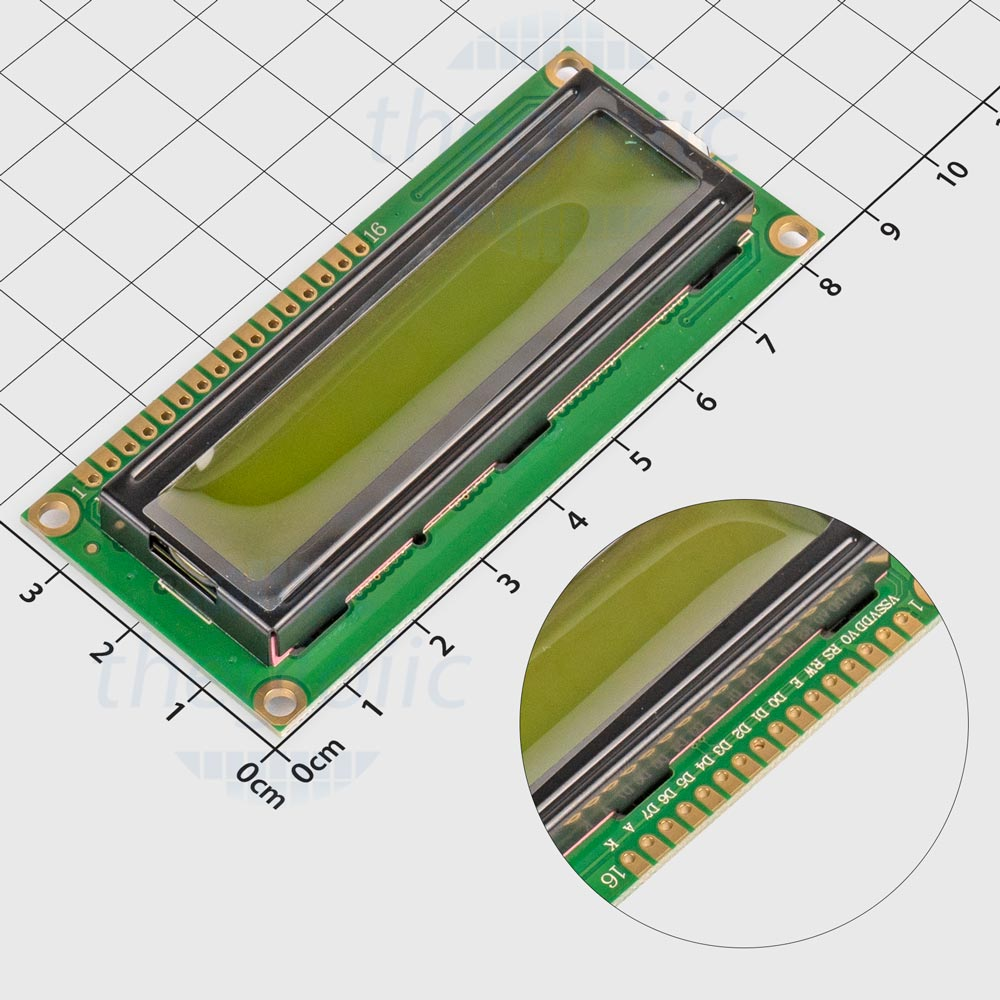
\includegraphics[width = 0.3\textwidth]{images/2.png}
    \caption{LCD 1602}
\end{figure}
\end{frame}

\begin{frame}
  \frametitle{Thông số linh kiện}
  \transdissolve
  \begin{itemize}
    \item Điện áp hoạt động (VCC): 5V DC (Thường hoạt động ổn định trong khoảng 4.7V - 5.3V).
    \item Dòng điện tiêu thụ: Khoảng 1mA (không đèn nền) và lên đến 20-30mA (có đèn nền).
    \item IC điều khiển (Controller): HD44780 hoặc tương đương.
    \item Khả năng hiển thị: 16 cột x 2 hàng (tối đa 32 ký tự).
    \item Kích thước điểm ảnh: 5x8 điểm (dot matrix) cho mỗi ký tự.
    \item Màu sắc: Thường là chữ trắng nền xanh dương hoặc chữ đen nền vàng xanh.
    \item Giao tiếp: Song song (Parallel) 4-bit hoặc 8-bit.
\end{itemize}
\end{frame}
\begin{frame}
  \frametitle{Thông số linh kiện}
  \begin{figure}[h!]
    \centering
    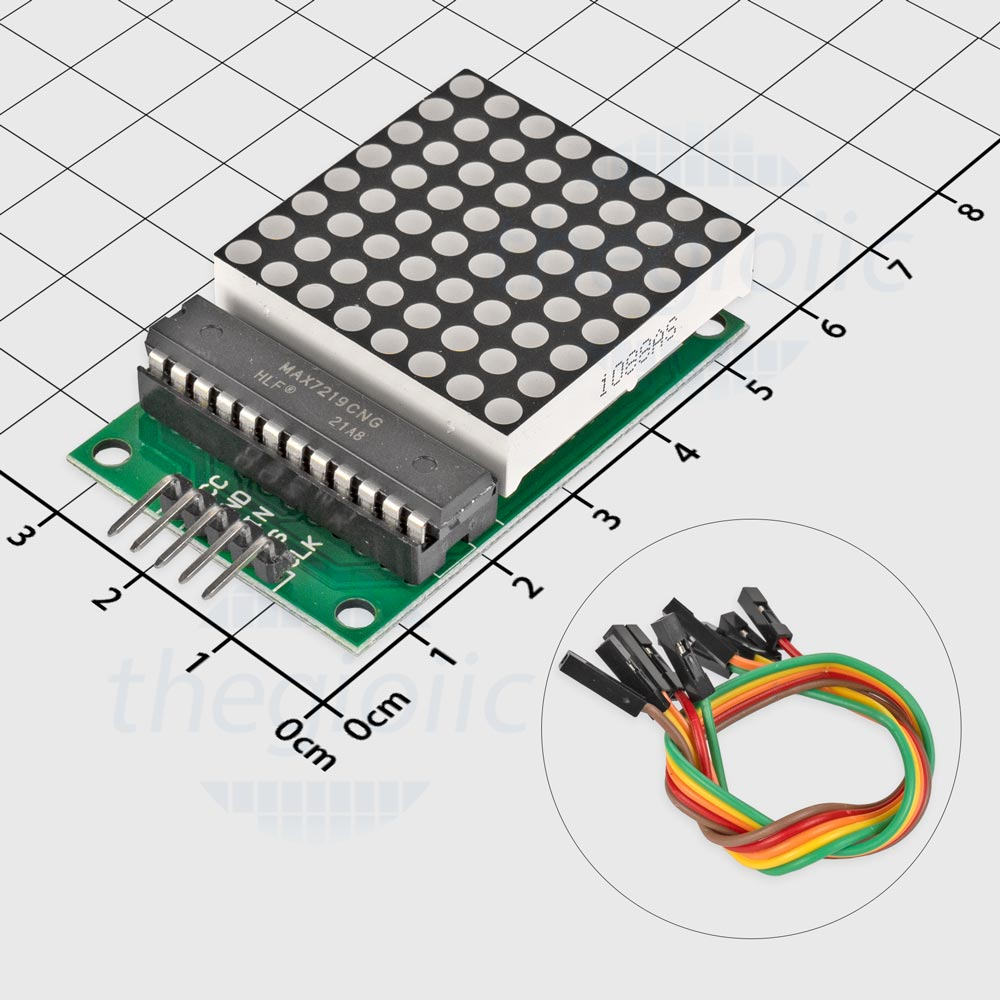
\includegraphics[width = 0.3\textwidth]{images/5.png}
    \caption{MAX7219 led matrix}
\end{figure}
\end{frame}

\begin{frame}
  \frametitle{Thông số linh kiện}
  \transdissolve
  \begin{itemize}
    \item IC điều khiển: MAX7219 (Driver hiển thị LED Cathode chung, đầu vào/ra nối tiếp).
    \item Màu sắc hiển thị: Đỏ (phổ biến nhất), Xanh lá, hoặc Xanh dương.
    \item Điện áp hoạt động: 4.0V - 5.5V DC (Khuyến nghị 5V).
    \item Giao tiếp: Serial Interface (Tương thích SPI) gồm 3 dây: DIN, CS (LOAD), CLK.
    \item Tần số xung nhịp tối đa: 10 MHz.
    \item Khả năng điều khiển: 1 IC MAX7219 điều khiển được 64 LED đơn (hoặc 1 ma trận 8x8, hoặc 8 LED 7 thanh).
    \item Điều chỉnh độ sáng: Kỹ thuật số (16 mức độ sáng thông qua thanh ghi nội).
    \item Dòng điện tiêu thụ: Tối đa khoảng 330mA (khi bật tất cả LED độ sáng cao nhất).
\end{itemize}
\end{frame}

\begin{frame}
  \frametitle{Thông số linh kiện}
  \begin{figure}[h!]
    \centering
    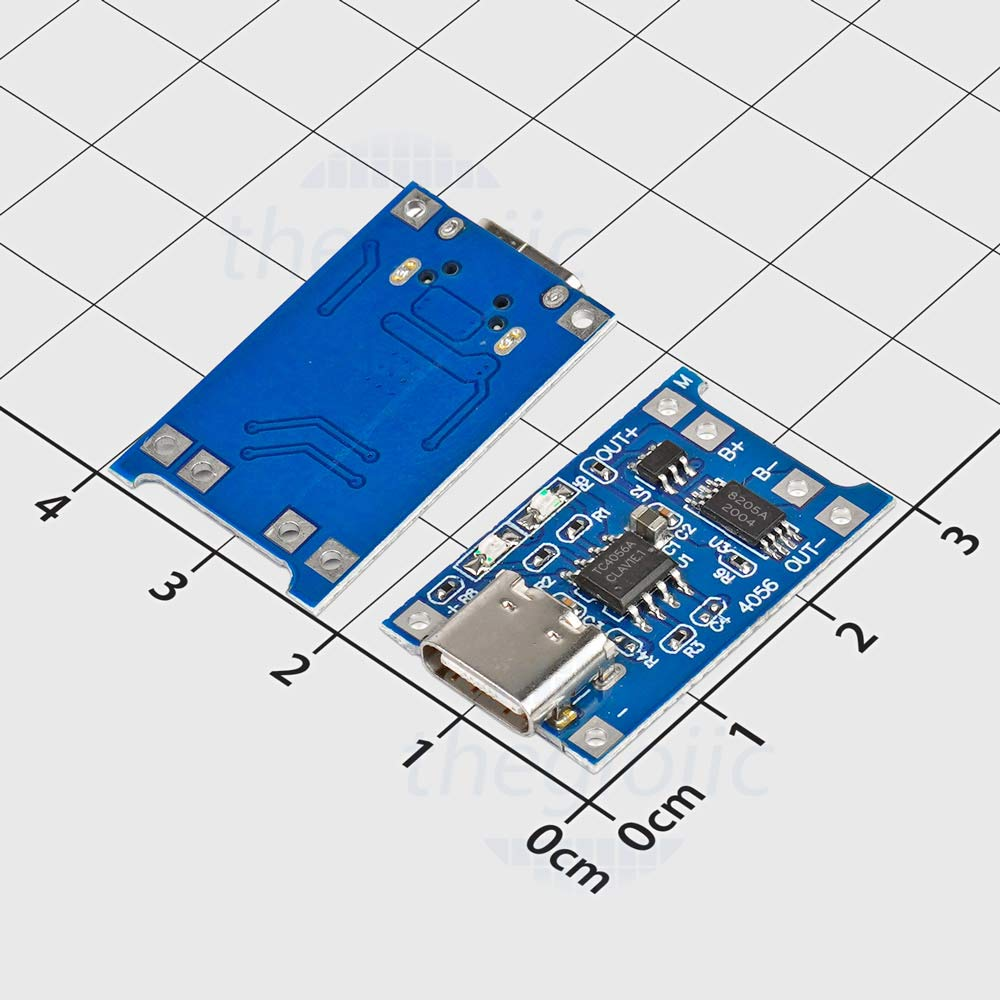
\includegraphics[width = 0.4\textwidth]{images/3.png}
    \caption{Mạch TP4056}
\end{figure}
\end{frame}

\begin{frame}
  \frametitle{Thông số linh kiện}
  \transdissolve
  \begin{itemize}
    \item Điện áp sạc: Cố định chính xác ở mức 4.2V.
    \item Dòng sạc tối đa: Có thể lập trình lên tới 1000mA (1A) chỉ qua một điện trở ngoài.
    \item Chu trình sạc: Tự động 3 giai đoạn: Sạc nhỏ giọt (khi pin < 2.9V), Sạc dòng không đổi (CC), Sạc áp không đổi (CV).
    \item Ngưỡng ngắt sạc: Tự động ngắt khi dòng sạc giảm xuống 1/10 dòng lập trình (C/10).
    \item Điện áp làm việc (VCC): 4V - 8V (Điển hình 5V).
    \item Bảo vệ tích hợp: Tự động giảm dòng khi IC quá nhiệt, khóa dưới áp (UVLO tại 3.7V).
    \item Dòng rò: Cực thấp (< 2$\mu$A) khi không có nguồn cấp, ngăn pin bị xả ngược.
\end{itemize}
\end{frame}
%---------------------------------------------------------
\section{PHẦN CỨNG}
%---------------------------------------------------------
\begin{frame}
\frametitle{Sơ đồ khối}
\begin{figure}[h!]
    \centering
    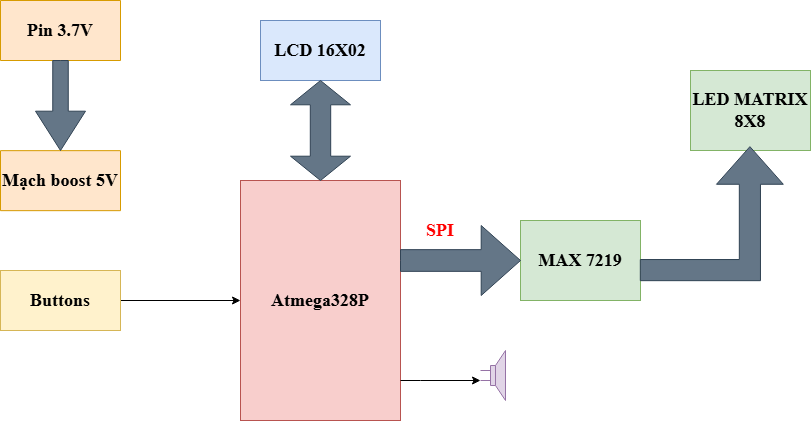
\includegraphics[width=.8\textwidth]{images/blockdiagram.png}
    \caption{Sơ đồ khối}
\end{figure}
\end{frame}

\begin{frame}
\frametitle{Sơ đồ nguyên lý}
\begin{figure}[h!]
    \centering
    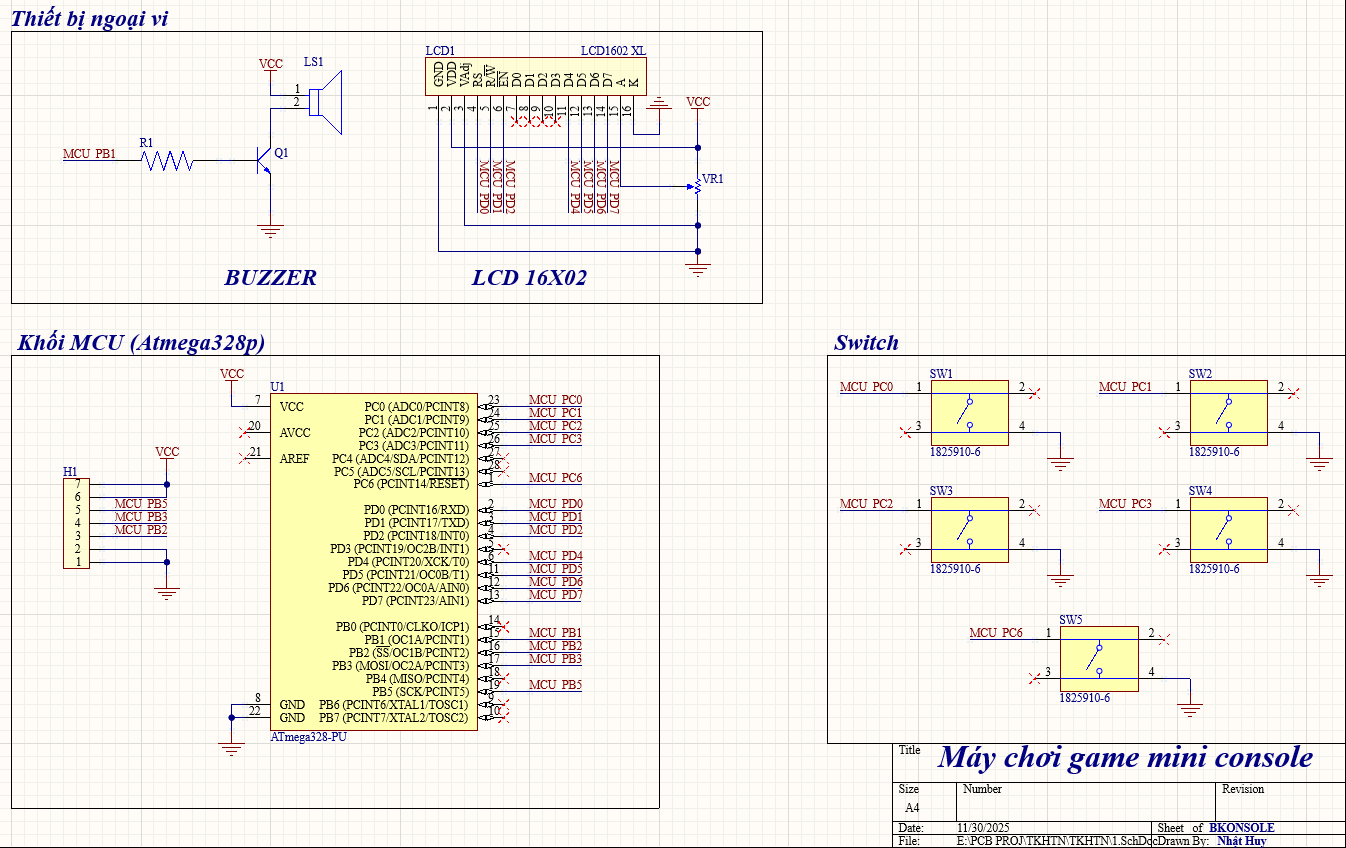
\includegraphics[width=0.7\textwidth]{images/SCHEM_main.png}
    \caption{Mạch nguyên lý của hệ thống}
\end{figure}
\end{frame}

\begin{frame}
\frametitle{Sơ đồ nguyên lý}
\transdissolve
\begin{figure}[h!]
    \centering
    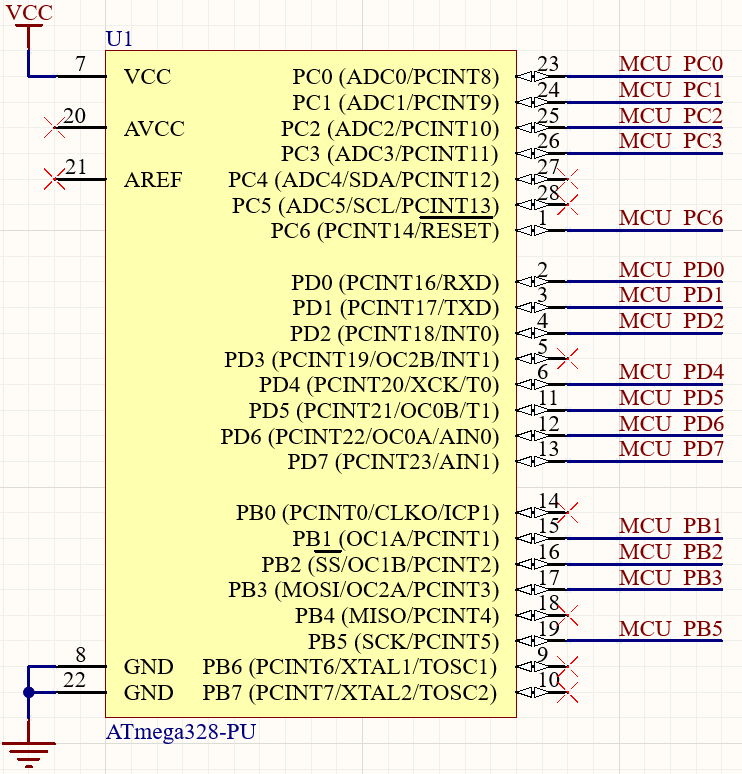
\includegraphics[width=.4\textwidth]{images/SCHEM_MCU.png}
    \caption{Khối vi xử lý trung tâm}
\end{figure}
\end{frame}

\begin{frame}
\frametitle{Sơ đồ nguyên lý}
\transdissolve
\begin{figure}[h!]
    \centering
    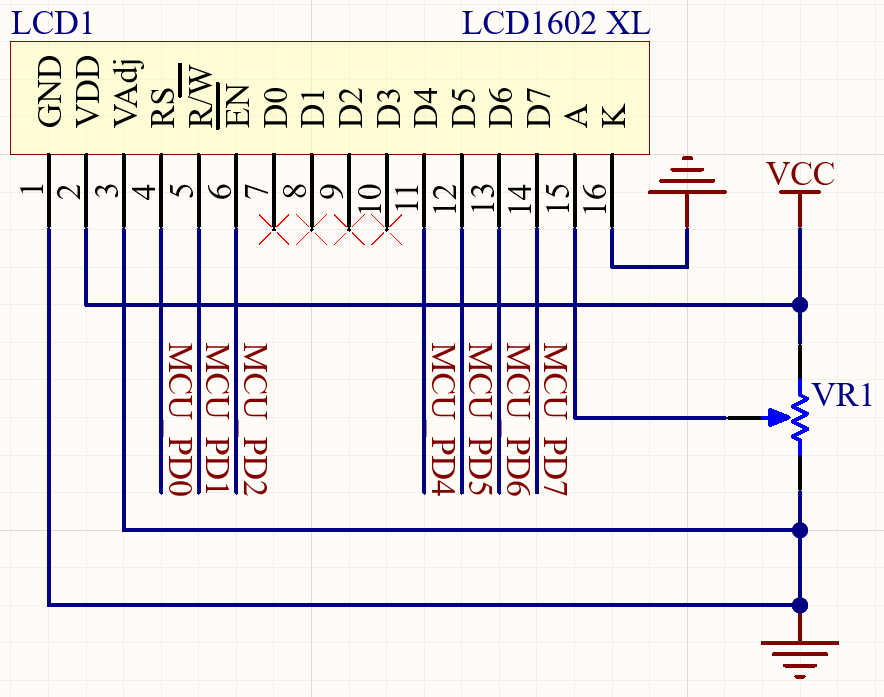
\includegraphics[width=.4\textwidth]{images/SCHEM_LCD.png}
    \caption{Khối giao tiếp LCD 1602}
\end{figure}
\end{frame}

\begin{frame}
\frametitle{Sơ đồ nguyên lý}
\transdissolve
\begin{figure}[h!]
    \centering
    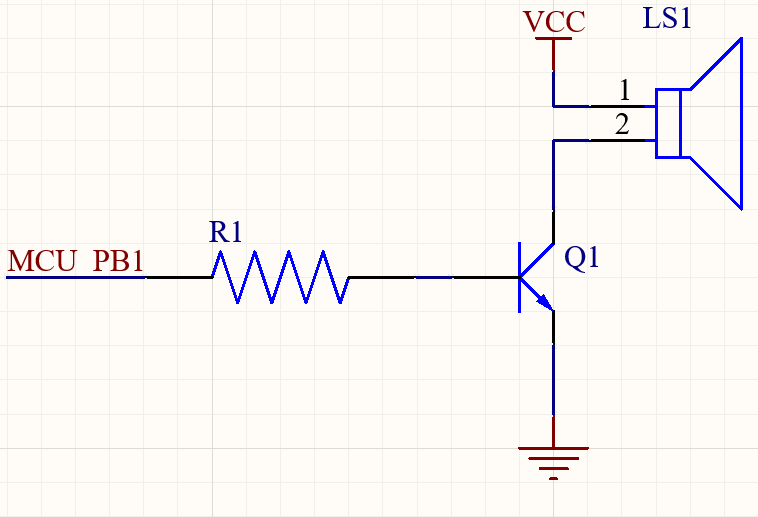
\includegraphics[width=.5\textwidth]{images/SCHEM_BUZZER.png}
    \caption{Khối giao tiếp Buzzer}
\end{figure}
\end{frame}

\begin{frame}
\frametitle{Sơ đồ nguyên lý}
\transdissolve
\begin{figure}[h!]
    \centering
    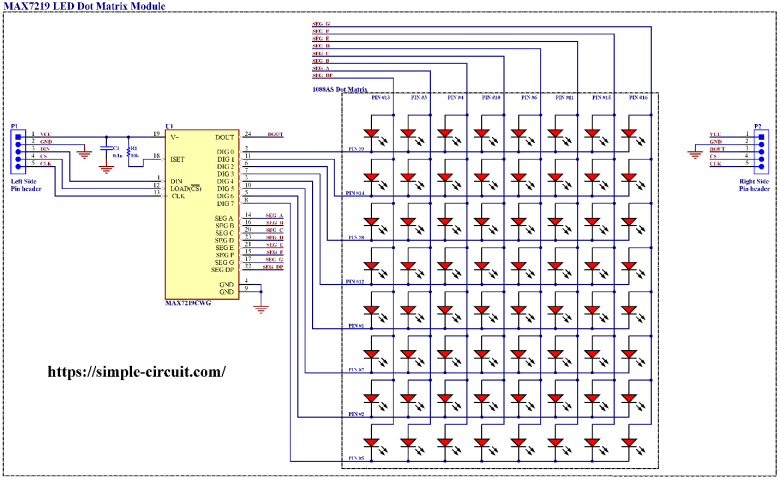
\includegraphics[width=.7\textwidth]{images/LED_MATRIX.png}
    \caption{Khối giao tiếp Led ma trận}
\end{figure}
\end{frame}

\begin{frame}
\frametitle{Sơ đồ nguyên lý}
\transdissolve
\begin{figure}[h!]
    \centering
    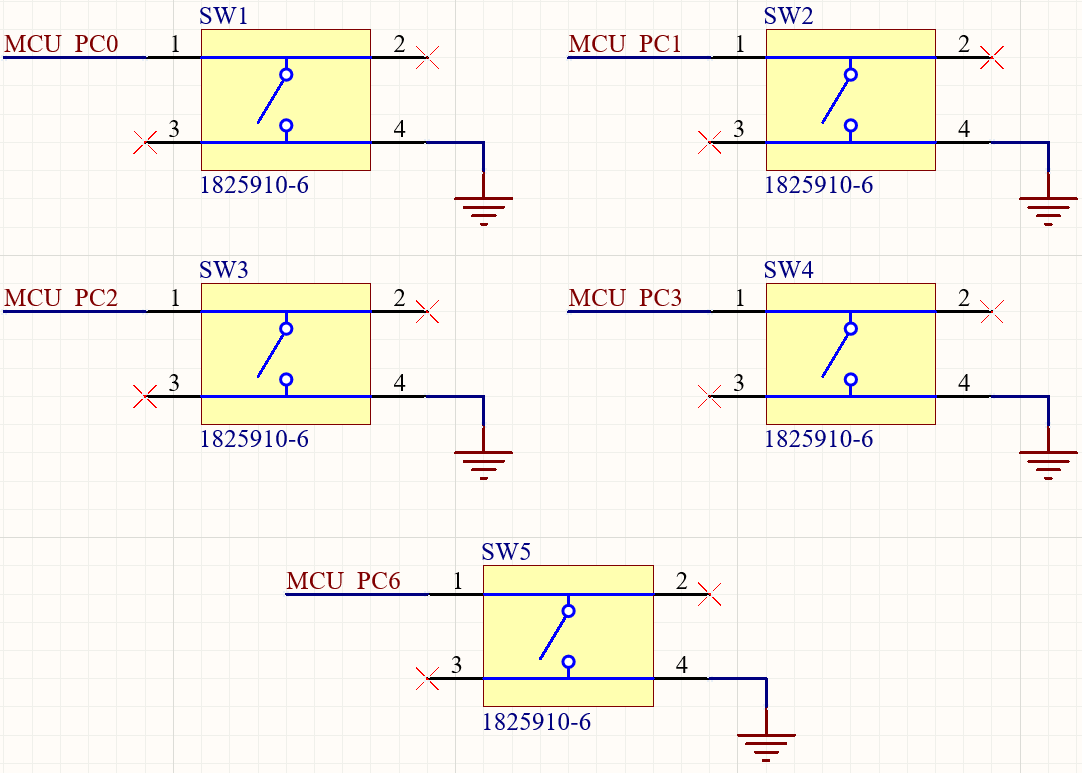
\includegraphics[width=.55\textwidth]{images/SCHEM_SW.png}
    \caption{Khối giao tiếp nút nhấn}
\end{figure}
\end{frame}

\begin{frame}
\frametitle{Sơ đồ nguyên lý}
\transdissolve
\begin{figure}[h!]
    \centering
    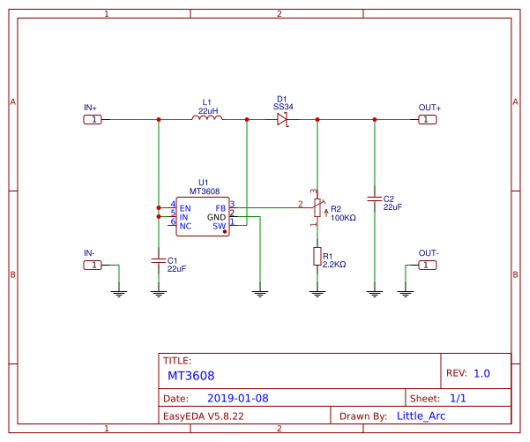
\includegraphics[width=.5\textwidth]{images/MT3608.png}
    \caption{Khối mạch tăng áp}
\end{figure}
\end{frame}

\begin{frame}
\frametitle{Sơ đồ nguyên lý}
\transdissolve
\begin{figure}[h!]
    \centering
    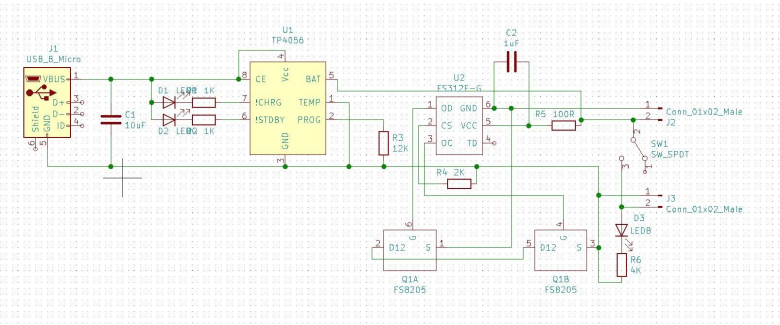
\includegraphics[width=.9\textwidth]{images/TP4056.png}
    \caption{Khối mạch sạc}
\end{figure}
\end{frame}
%---------------------------------------------------------
\section{PHẦN MỀM}
%---------------------------------------------------------
% Take away
% Contact
% Thank
\begin{frame}{Lưu đồ giải thuật tổng quát}
\begin{figure}[h!]
    \centering
    
\includegraphics[width=.7\textwidth]{images/main_struct.png}
    \caption{Lưu đồ giải thuật tổng quát}
\end{figure}
\end{frame}

\begin{frame}{Lưu đồ giải thuật game snake}
\begin{figure}[h!]
    \centering
    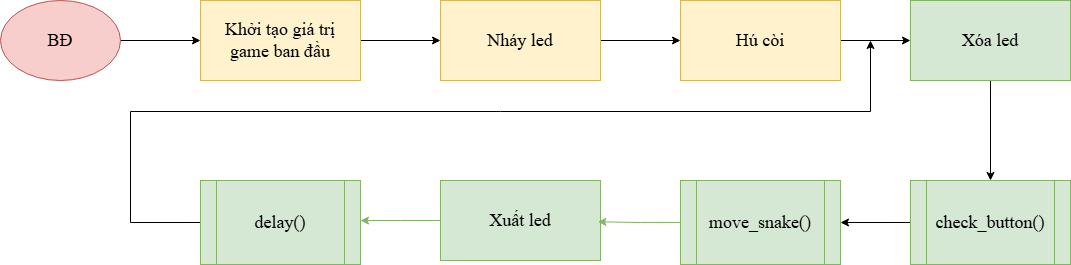
\includegraphics[width=.9\textwidth]{images/6.png}
    \caption{Lưu đồ giải thuật game snake}
\end{figure}
\end{frame}

\begin{frame}{Lưu đồ giải thuật game pickel ball}
\begin{figure}[h!]
    \centering
    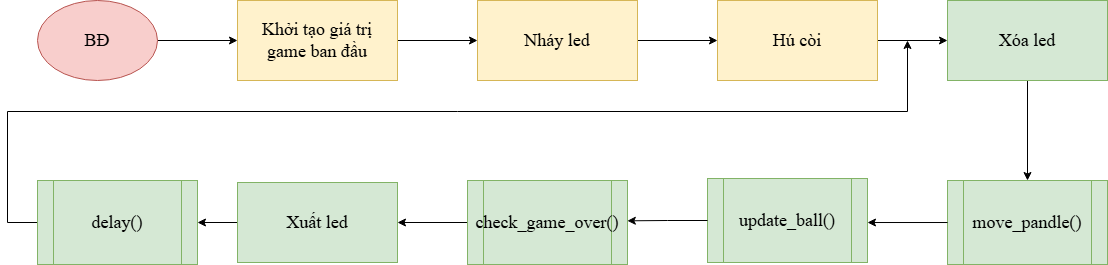
\includegraphics[width=.9\textwidth]{images/7.png}
    \caption{Lưu đồ giải thuật game pickel ball}
\end{figure}
\end{frame}
%---------------------------------------------------------
\section{KẾT QUẢ THỰC HIỆN}
%---------------------------------------------------------
\begin{frame}
\frametitle{Kết quả thiết kế qua Altium}
\begin{figure}[h!]
    \centering
    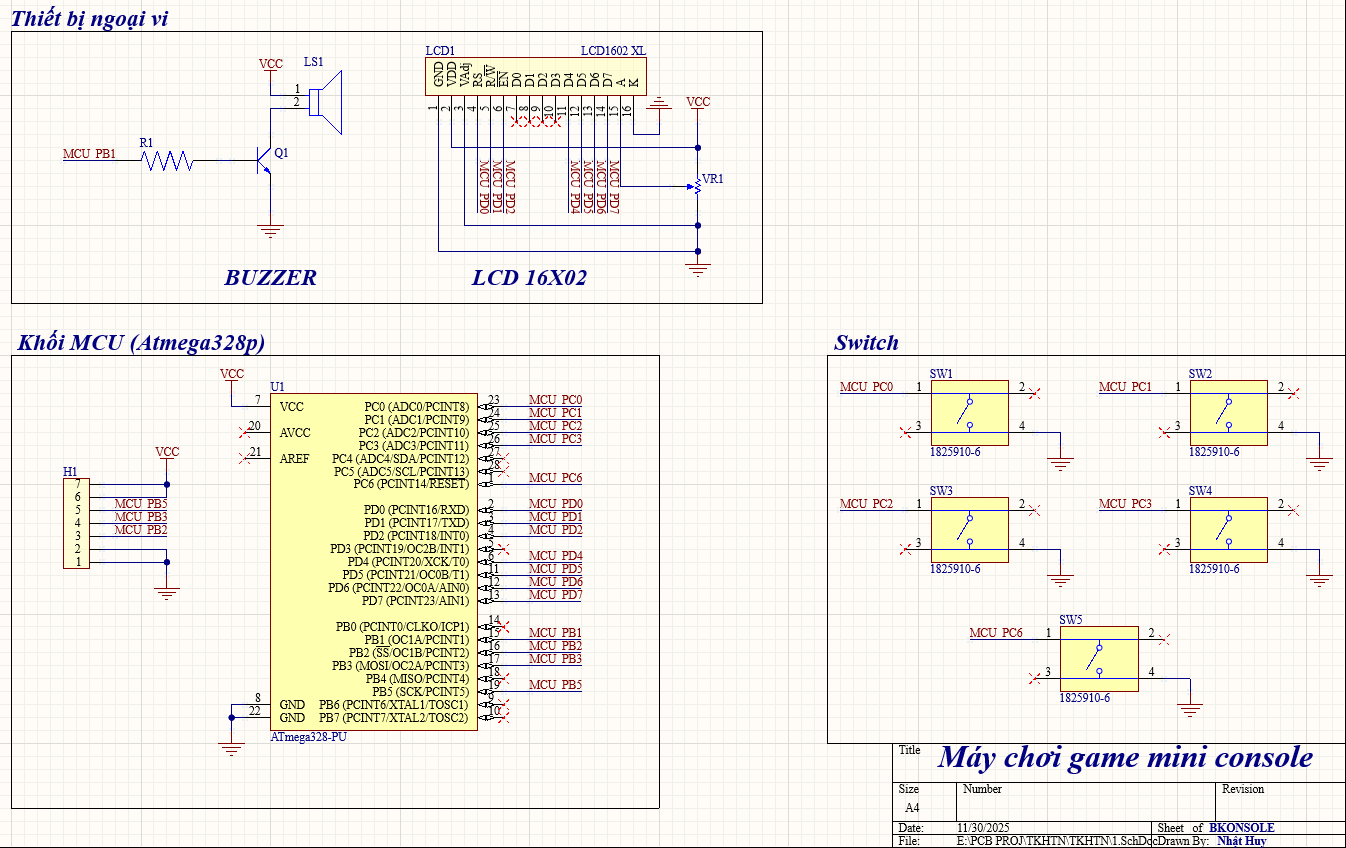
\includegraphics[width=0.7\textwidth]{images/SCHEM_main.png}
    \caption{Mạch nguyên lý của hệ thống}
\end{figure}
\end{frame}

\begin{frame}
\frametitle{Kết quả mô phỏng qua Altium}
\begin{figure}[h!]
    \centering
    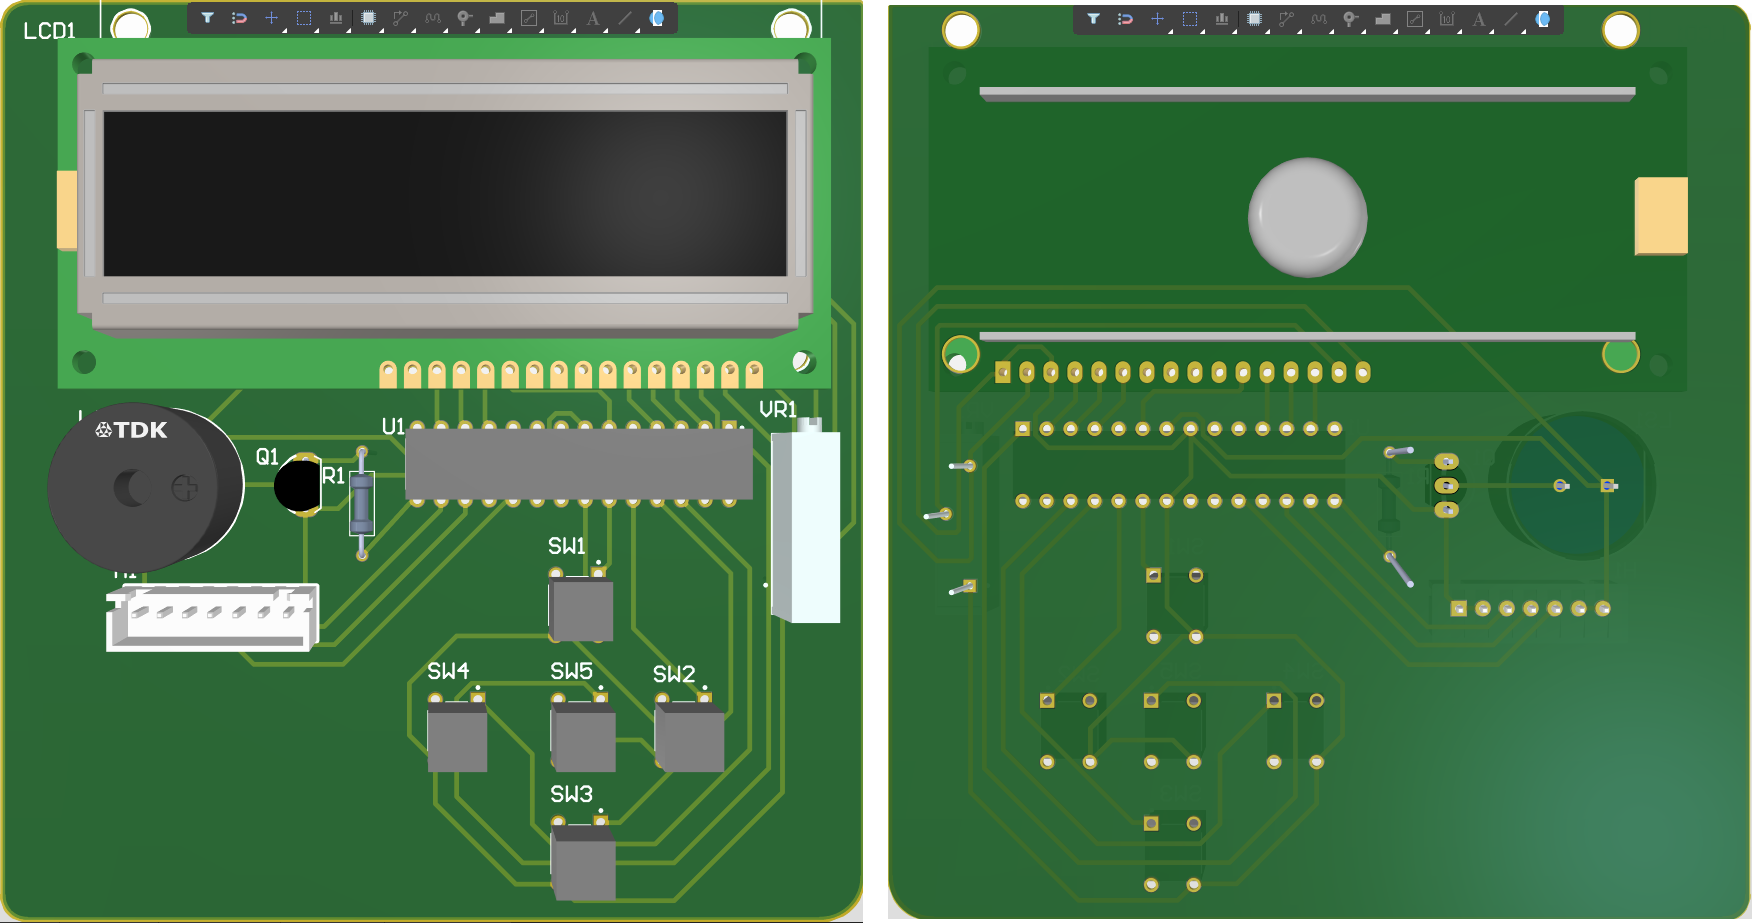
\includegraphics[width=.8\textwidth]{images/SCHEM_3D.png}
    \caption{Mạch in 3D (trước và sau) của hệ thống}
\end{figure}
\end{frame}

\begin{frame}
\frametitle{Kết quả gia công phần cứng}
\begin{figure}[h!]
    \centering
    \includegraphics[width=.4\textwidth]{images/demo.png}
    \caption{Kết quả gia công phần cứng}
\end{figure}
\end{frame}

\setbeamertemplate{footline}{}
\begin{frame}
    \centering
    \vspace{1cm}
    \textbf{\Huge{- THE END - }}\\
    \vspace{0.2cm}
    \textit{\Large{Cảm ơn thầy và các bạn đã chú ý lắng nghe}}\\
\end{frame}
\end{document}